\documentclass[9pt,twocolumn,twoside]{idsi}
% Defines a new command for the horizontal lines, change thickness here
\newcommand{\HRule}{\rule{\linewidth}{0.5mm}} 
\usepackage{listings}
\renewcommand{\headrulewidth}{2pt}
\fancypagestyle{plain}{%
  \fancyhead[L]{
    \begin{tabular}{ll}
%        
\includegraphics[scale=0.15]{figs/ncsa_vertical} 
    \end{tabular}       
  }
  \fancyhead[C]{
      	\begin{tabular}[m]{c}
		  	\fontsize{20}{20} Illinois Data Science Initiative    	
		\end{tabular}
  }

  \fancyhead[R]{
    \begin{tabular}{ll}
%	  	
\includegraphics[scale=0.125]{figs/ill}  		
  	\end{tabular}
  }
  
  \fancyfoot[C]{\thepage}
}
\pagestyle{plain}
\def \report_title {Machine Learning Model Selection Algorithm on Spark's MLlib}
\author[1]{Jacob Trauger}
\author[1]{Sahil Bhatt}
\author[2]{Professor Robert J. Brunner}
\affil[1]{Illinois Data Science Initiative}
\affil[2]{Laboratory for Computation, Data, and Machine Learning}
\title{Machine Learning Model Selection Algorithm on Spark's MLlib}

\begin{abstract}
Model selection for machine learning algorithms is a useful tool to decide which machine learning technique to use for data analysis. This model selection algorithm for Apache Spark's MLlib library allows a user to select and use the most suited machine learning algorithm without requiring the user to have knowledge of the intricacies involved in machine learning theory.
\end{abstract}

\begin{document}

\coverpage{Machine Learning Model Selection Algorithm on Spark's MLlib}{Jacob Trauger \\ Sahil Bhatt\\Professor Robert J. Brunner}

\maketitle


\section{Introduction} 
Machine learning is a very useful tool for data analysis, but utilizing it requires an understanding of complex mathematics and statistics. This is why many libraries, like Scikit-learn \cite{scikit_learn} and Apache Spark's MLlib \cite{spark_mllib}, abstract the complex mathematics away into simple functions that can be used given a basic understanding of the library's language. These libraries are immensely helpful for simplifying the process of using machine learning techniques on a dataset. However, the problem remains of choosing the correct technique or machine learning model to use with a dataset. Due to the vast number of machine learning algorithms each with their own specific set of parameters and assumptions, this can be a rather difficult problem. 
This paper outlines a solution in the form of a model selection algorithm in Apache Spark's MLlib that, given a few parameters, will select the best algorithm for the programmer and run it on the dataset given. 

\section{Assumptions}
It is assumed that users have 
\begin{itemize}
\item Spark/MLlib installed on their computer/cluster
\item Basic understanding of python
\end{itemize}

\section{About Machine Learning}
A machine learning algorithm is an abstract term given to all algorithms that predict population parameters from a given set of data. There are three main categories of machine learning: supervised, unsupervised, and reinforcement learning algorithms. Spark's MLlib \cite{spark_mllib} (and therefore this model selection algorithm) only supports algorithms for supervised and unsupervised learning. Thus, due to this restriction, these categories are going to be the only categories mentioned in the rest of the paper, but other types of machine learning algorithms do exist. 

\subsection{Supervised Learning}
Supervised algorithms are used when the data has some label attached to it. For example, if there was a dataset of an arbitrarily large amount of six sided die rolls, where the even-numbered rolls were considered wins and the odd-numbered rolls were considered losses, the dataset would need to have label-feature pairs where the label represents a win or a loss (usually 0 for loss or 1 for win) and the feature would be the die roll.

 Table \ref{tab:Die-tosses} shows an example table. 
\begin{table}[htbp]
\centering
\caption{\bf Probability Space of Die Toss}
\begin{tabular}{ccc}
\hline
Die Value & Label & Label-Feature Pair \\
\hline
$X = 1$ & $0(Loss)$ & $(0,1)$ \\
$X = 2$ & $1(Win)$ & $(1,2)$ \\
$X = 3$ & $0(Loss)$ & $(0,3)$ \\
$X = 4$ & $1(Win)$ & $(1,4)$ \\
$X = 5$ & $0(Loss)$ & $(0,5)$ \\
$X = 6$ & $1(Win)$ & $(1,6)$ \\
\hline
\end{tabular}
  \label{tab:Die-tosses}
\end{table}

In this experiment, if the data was sent through a supervised learning algorithm and it was asked to predict the label of a die roll of 2, it would output a 1 and, if it was asked to predict the label of a 3, it would output a 0. Table \ref{tab:Die-predict} shows an example table. The algorithm here would be a supervised classifier because the data is supervised and the prediction is being classified into groups. 

\begin{table}[htbp]
\centering
\caption{\bf Die Prediction}
\begin{tabular}{ccc}
\hline
Die Value & Predicted Label \\
\hline
$X = 2$ & $1$ \\
$X = 3$ & $0$ \\
\hline
\end{tabular}
  \label{tab:Die-predict}
\end{table}

There is also supervised regression which, instead of classifying on a finite number of labels, will attempt to predict an exact value. Supervised regression will essentially create a function from the feature space to the label. It is the same concept as classification just with more precision, because instead of breaking up the label space into classes it will try to predict an exact value for the output. One such use of a regression algorithm is trying to predict the exact weight of a person off their height, sex, and average ingested calories.

\subsection{Unsupervised Learning}
The last type of machine learning algorithm used in this paper is unsupervised learning. Unsupervised learning does not need a the label in order to predict the given parameters. Instead it is able to guess population parameters by looking at the structure of the data. The model selection algorithm only includes support for unsupervised clustering, so only that will be covered in this report. Clustering can be thought of much like classifying except there is no label. Instead, it looks at the parameters given and is able to predict which data points are in the same group. An example could be of the clusters of businesses in a town. Given a location dataset of the businesses in a town, an unsupervised learning algorithm should be able to cluster businesses together and, given a new business location, be able to predict what cluster it is in. Unsupervised learning is useful because it finds the underlying structure of the data. 

One use of an unsupervised learning algorithm would be political party classification. If there was data on an individual's voting patterns, and this data was then clustered, the clustered data can be analyzed to see if clusters of people have an affinity to vote for a certain political party. 
\begin{figure}[htbp]
\centering\fbox{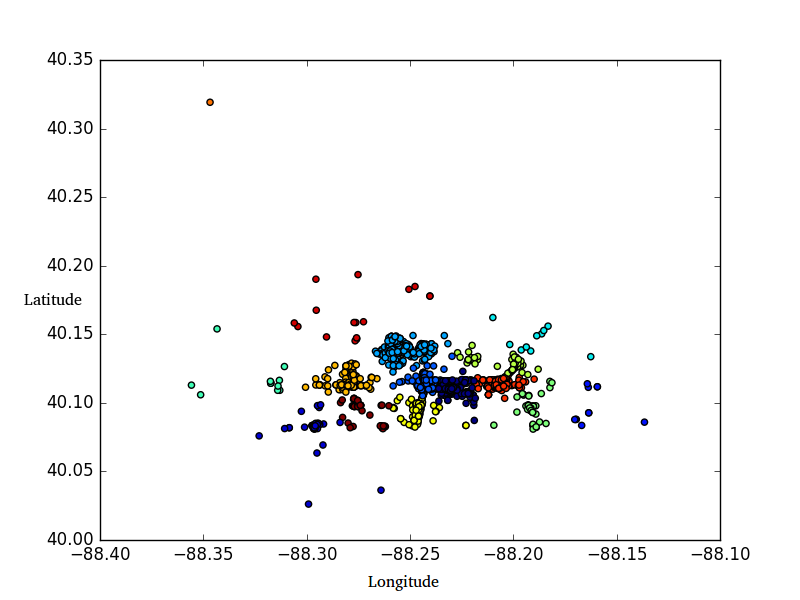
\includegraphics[width=\linewidth]{C-Uyelp.png}}
\caption{A k-means algorithm ran on a yelp restaurant dataset for the Champaign-Urbana, IL area}
\label{fig:KMeans}
\end{figure}



\section{MLlib Model Selection Algorithm} \label{algo}
For this paper, a model selection algorithm has been derived that given parameters, will pick the an appropriate model for the user. This will help beginner Spark programmers pick an appropriate machine learning model without a deep understanding of the machine learning algorithms. The model selection algorithm is based on Scikit-Learn's Cheat Sheet \cite{scikit_learn}, which is a flowchart used to pick the most optimal machine learning algorithm given a dataset. The algorithms themselves are taken from Apache Spark's MLlib library. The algorithms currently used in this model selection are:

\begin{itemize}
\item Supervised Classification
	\begin{itemize}
	\item Naive Bayes - Uses Bayes Theorem (eq \ref{eq:Bayes}) to try and find the label given the features. The reason why it is naive is because it assumes independence between all of the features.
    \begin{equation}
    P(A|B) =\frac{P(A \cap B)}{P(B)} = \frac{P(B|A) \cdot P(A)}{P(B)}
    \label{eq:Bayes}
    \end{equation}
	\end{itemize}
\item Supervised Regression
	\begin{itemize}
	\item Linear Regression - Fits a linear function through the data to predict the label given the features. It does this by minimizing the square of the difference between the predicted point and the actual point.
    \item Ridge Regression  - Creates a regression model which performs L2 regulation, which is based on minimizing the square of the weights along with the loss function. The weights of the function are the coefficients given to each feature to try to predict the label value. Minimizing the weight helps in preventing overfitting which is talked more in-depth in \ref{modelMetrics}\ref{overfitting}
    \item Lasso Regression - Creates a regression model which performs L1 regulation which is based on minimizing the absolute value of the weights along with the loss function.
	\end{itemize}
\item Unsupervised Clustering
	\begin{itemize}
	\item K-Means - Creates partitions of data into k clusters where each data point belongs to the cluster with the closest center.
	\end{itemize}
\end{itemize}

The model selection algorithm takes at minimum 5 parameters in this order: 
\begin{enumerate}
\item The dataset(either a JSON or CSV formatted file). Currently the algorithm only supports files on HDFS.
\item Whether the data is supervised/unsupervised.
\item Whether it should be a regression/classifier/clustering algorithm.
\item The parameter trying to be guessed (if supervised this is the label name).
\item The other parameters that are being used to predict the first parameter.
\end{enumerate}

When the program is run, the first thing it does is filter the dataset so only the parameters wanted are left. This happens in different ways for the JSON or CSV files due to their inherent differences in storing data.

For JSON datasets, the $jsonFilterAndMap(dataRDD, paramsArray)$ function filters the data so that only the parameters that are wanted are left, and these parameters are left in such a way that the position of the values are in the same place as the keys are in the array. This is done easily with JSON files because JSON is stored as key, value pairs. Therefore it is only necessary to iterate through the $params$ array and keep them in the RDD.


CSV files are harder to work with due to there being no key value pairs. The $csvFilterAndMap(dataRDD, paramsArray)$ function is what filters CSV files. This function creates a dictionary from $paramsArray$ to the position it corresponds to in the CSV file. Then, using this dictionary, the program filters the RDD by creating a key value pair, where the key is the parameter and the value is the value of $dataRDD$ at the position $dictionary[key]$.

After the data is filtered and mapped, given whether or not it is a supervised classifier, supervised regressor, or an unsupervised dataset, it will narrow down the algorithms to a few algorithms to test. For supervised learning algorithms, it will test each algorithm on a relatively small (30\% of actual size) randomized subset of the dataset (to speed up the runtime) and then it will choose the best algorithm  based on which machine learning algorithm  yields the most desirable results on the smaller dataset. 30\% is chosen as a heuristic number because it is small enough to have each algorithm run in a reasonable time and it is large enough where the tendencies between the algorithms should start to show without overfitting (overfitting is explained in \ref{modelMetrics}\ref{overfitting}). Once it chooses the best model for the smaller dataset, then it will retrain that model and then predict the testing data from a random sampling (80\% training, 20\% testing) of the entire dataset instead of small subset of the dataset.

For unsupervised learning algorithms, it also trains on the smaller dataset through many different numbers of clusters and then chooses the best algorithm with the optimal amount of clusters and returns those values. Then the selected model is trained on the dataset. Unlike supervised learning, unsupervised learning does not need labels. Instead, it clusters the data and selects the best number of clusters by finding at what amount of clusters is the point of dimishing returns in the within set sum of squares error (WSSSE) function, which is explained in \ref{modelMetrics}\ref{wssse}

Below is the code for choosing which regression model works best. The performRegression function trains the models on the sample data and returns which model is the best given the sample data. 


\begin{lstlisting}[language=Python]
def performRegression(data):
        training, test = data
        	.randomSplit([.8, .2])
            
        lasso = performLasso(training)
        linReg = performLinearRegression(training)
        ridgeReg = performRidgeRegression(training)

        lassoTest = (test.map(lambda x: x.label)
        	.zip(lasso.predict(test.map(
            lambda x: x.features))))
        linTest = (test.map(lambda x: x.label)
        	.zip(linReg.predict(test.map(
            lambda x: x.features))))
        ridgeTest = (test.map(lambda x: x.label)
        	.zip(ridgeReg.predict(test.map(
            lambda x: x.features))))

        lassoMetrics = RegressionMetrics(
        	lassoTest.map(
            lambda x: (x[0], float(x[1]))))
        linMetrics = RegressionMetrics(
        	linTest.map(
            lambda x: (x[0], float(x[1]))))
        ridgeMetrics = RegressionMetrics(
        	ridgeTest.map(
            lambda x: (x[0], float(x[1]))))

        lassoValue = lassoMetrics
        	.rootMeanSquaredError
        linRegValue = linMetrics
        	.rootMeanSquaredError
        ridgeRegValue = ridgeMetrics
        	.rootMeanSquaredError

        if(lassoValue < linRegValue 
        	and lassoValue < ridgeRegValue):
                return "lasso"
        if(linRegValue < lassoValue 
        	and linRegValue < ridgeRegValue):
                return "linear"
        return "ridge"
\end{lstlisting}





\section{Model Selection Metrics} \label{modelMetrics}

\subsection{Accuracy And Precision}
In order to choose which model works for a given set of parameters and a given dataset, the accuracy of each model is evaluated. Accuracy is tested through training the data of a particular dataset through a machine learning algorithm and then testing data to see if the algorithm can "predict" correctly. For example, going back to the Table \ref{tab:Die-predict} example, if Naive Bayes is used to train a model to predict the label based on the die-value, the model's output would be in the form of a confusion matrix. 

A confusion matrix is used to describe the behavior of classification models such as Naive Bayes. This matrix contains information regarding the accuracy, precision, misclassification/error rate, and many other factors. These matrices represent each class where the rows are the actual class and the columns are what the model predicted. 
\begin{verbatim}

Confusion Matrix
[[ Predicted 1 Actually 1.		Predicted 2 Actually 1.]
 [ Predicted 1 Actually 2.  	Predicted 2 Actually 2.]]

\end{verbatim}

In the example confusion matrix below, the Naive Bayes algorithm is used to predict HelpfulnessDenominator based on Score and HelpfulnessNumerator in an Amazon reviews dataset. HelpfulnessDenominator is the number of people who rated a review as unhelpful, HelpfulnessNumerator is the number of people who rated a review to be helpful, and the Score is the score (out of 5) the reviewer gave the product. The columns are the predicted values and the rows are the actual values for the labels. So in this testing data, 52802 of the data is correctly predicted as a HelpfulnessDenominator of 0, while 4573 are incorrectly predicted as a 1 when HelpfulnessDenominator is actually 0, etc. In general, the more values on the left-to-right diagonal means the better the prediction is because those are where the predicted values and actual values align. There are more than 5 different classifications in the actual results but the only first 5 are listed below because after 5 the matrix gets sparse.

\begin{verbatim}

Testing Data Confusion Matrix
[[ 53802.  4573.  1198.  411.  211.  142.  76. ...]
 [     0. 18218. 10102. 2037.  533.  274. 169. ...]
 [     0.     0.  1118. 4089. 2729.  744. 281. ...]
 [     0.     0.     0.  342.  609. 1493. 478. ...]
...]
Accuracy: 0.6502161003548965

\end{verbatim}

Above the data confusion matrix and data accuracy are shown for the testing data. The dataset is split into two sets: training data, that is used to train the model, and testing data, that is used as a "test" for the model to see how accurate it is. By convention, machine learning researchers split the dataset into no more than 80\% for training and the rest (20\%) will be used for testing. 

The data accuracy gives us the percent of data which the model predicted correctly. Only the outputs for the testing data are given because usually the training data has a higher accuracy due to random correlations in the training data that do not appear in the actual population. These random correlations will make it predict slightly off because it will be predicting on things which are independent of the actual parameter. This is called overfitting and is covered more in section \ref{modelMetrics}\ref{overfitting}. Therefore, only the testing data is shown to give a more general and non-biased report of how the model performed.

\subsection{Loss Factor} \label{lossFactor}

\subsubsection{Root Mean Squared Error (RMSE)} \label{rmse}

For regression algorithms, explained variance should be maximized and the root mean squared error (RMSE) should be minimized. 
The explained variance is the amount of variance in the data that is explained by the model. Let X be the observed value, \^{X} be the predicted value, and n be the amount of predictions made. Then the root mean squared error is the calculated by 

\begin{equation}
RMSE =\sqrt[]{\frac{\sum_{i=1}^{n} (\hat{X_i} - X_i)^2}{n}}
\label{eq:rmse}
\end{equation}

This equation finds the average distance between the actual value and the predicted value\cite{rms_error}. So, if this value was large, then on average there would be a large distance between the predicted value and the observed value, which is unwanted and an indicator of low accuracy.



\subsubsection{Within Set Sum of Squares Error (WSSSE)} \label{wssse}
Clustering is different because, unlike classification and regression, there is no explicit checking. Instead, the goal of a clustering algorithm is to split the data into as few distinct clusters as possible. In order to find the k value which most effectively distinguishes the clusters, the algorithm must be run for a range of the k values, and at each iteration the within set sum of squares error (WSSSE) should be recorded. Let \^{X} be a member in a group, X be the center of that group, m be the total amount of points that are in the group, and N be the number of groups. Then the within set sum of squares error is calculated by

\begin{equation}
WSSSE =\sqrt[]{\frac{\sum_{n=1}^{N}\sum_{i=1}^{m} (\hat{X_{\text{ni}}} - X_{\text{ni}})^2}{n}}
\label{eq:wssse}
\end{equation}

This allows for the model to get the average distance each point is away from the center of its respective group. Unlike the RMSE, the goal is not to minimize the formula, but find the point of diminishing returns. Although adding more and more groups will minimize the WSSSE, this will also start to break apart groups of points that should be together. That is why the point of diminishing returns is used; it allows the maximum size for each cluster while being small enough that each group is actually clustered together. In the model selection algorithm, the point of diminishing returns is defined as the point when increasing the k value will result in a change of less than (.05 * |(WSSSE at k=1) - (WSSSE at k=2)|). This was chosen as it is easy to calculate and, through trial and error, is fairly accurate.

\subsubsection{Overfitting} \label{overfitting}

Another way to test the effectiveness of a machine learning model is to make sure that the model is not overfitting the data. A model is considered overfitted when it adapts to the patterns in the training data to an extent that it is no longer representative of the real world data.

\begin{figure}[htbp]
\centering
\fbox{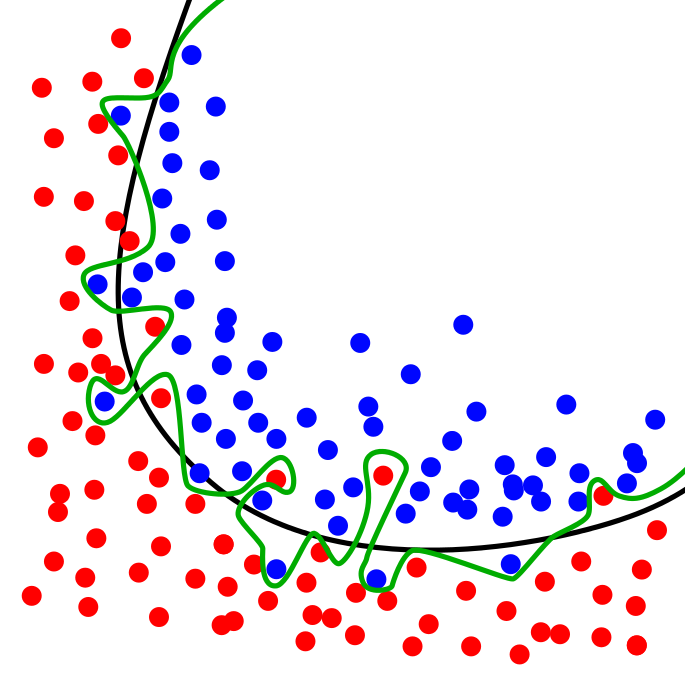
\includegraphics[width=\linewidth]{overfitting.png}}
\caption{Overfitting visual \cite{overfitting_image_bib}}
\label{fig:overfittingImage}
\end{figure}

In figure \ref{fig:overfittingImage}, there is an example of an overfitted model. The green line is the regression function predicted by the overfitted model. It takes into account all the "noise" in the test data and uses it to predict the regression function.  This is considered a bad model compared to the "regularized" model which is illustrated in a black line. The "regularized" model fits the data and makes sure that the data is not overfitted. 

This is especially important as regression models which are overfitted are suboptimal. That is why supervised regression algorithms, such as lasso and ridge regression, use regularization to construct their models. This ensures that the data is neither overfitted nor underfitted meaning that the model fits both the training and testing dataset. However, regularizing functions often have the drawback of having a lower accuracy than other models used with the same data.%"and it is just right" 

\begin{figure}[h!tbp]
\centering
\fbox{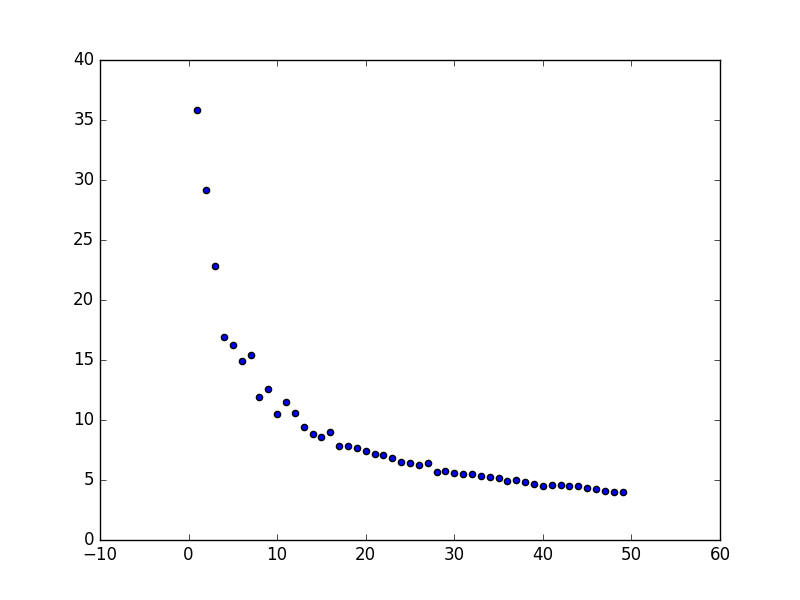
\includegraphics[width=\linewidth]{WSSSE.png}}
\caption{A scatter plot of the WSSSE values of for the dataset used in Fig \ref{fig:KMeans}}
\label{fig:WSSSE}
\end{figure}

\section{Workflow}
One can interact with the model through any medium that can run a spark program. In this example though, a bash shell will be used as this medium. The model selection program is run using the following code:
\begin{lstlisting}
pyspark modelSelections.py DATASET TYPE \
CLASS_OR_REG OUTPUT_PARAM OTHER_PARAMS
\end{lstlisting}
(Note: the slash denotes that these should all be on the same line; do not include the slash.)
After it is finished running there will be a results.txt and, in hdfs, there will be a new directory named theModel. The results.txt file shows how the model did on the training data (it includes the appropriate accuracy and precision data along with the appropriate loss factors), and the theModel directory stores the model for future use.

\section{Limitations}
There are some limitations to this model selection. One such limitation is that there are only the few algorithms in the model selection for each different type of machine learning. Also, the models have to be generalized so that they fit all cases; this means that the dataset has to be simplified down to its bare minimum and therefore forgoes a lot of possibilities of training the data in other ways. An example of this limitation is text data. Since there is no universal way to convert text data into meaningful numerical data, a model supporting text data could not be used. This algorithm also does not support learning on anything other than the parameters given. This model cannot predict a outcome based on a ratio of parameters. There is a possibility that one could learn on all of the parameters wanted in the ratio and then the computations to obtain the ratio, but this has not been tested.

\section{Further Development/Research}
Increasing the number of algorithms which are tested could help users choose a machine learning algorithm which better suits their data, but this comes with a drastic increase in runtime. Another advancement is to change the selection algorithm so that the data does not need to be run on each machine learning algorithm. There could be some way that, given the parameters (which may need to expanded if needed), one model might work better in that situation without needed to run all of the possible algorithms. There are also alternative, more in depth functions and algorithms that measure how accurate and reliable a machine learning algorithm is. One or more of those could be implemented to make the choosing of the algorithm more precise.

\section{Conclusion}
This model selection algorithm is a powerful tool for a beginner in machine learning. It allows the programmer to use five different algorithms in a way that tailors to each one.

If the dataset is labeled and classification is wanted, then Naive Bayes is a simplistic yet powerful machine learning algorithm that will work. When it was ran on the Amazon review dataset it predicted fairly accurately as seen by the confusion matrix. Even with the assumption of independence it still works very well; it is very versatile and what it lacks in accuracy it makes up for in reliability. 

Having multiple regression algorithms adds more reliability and accuracy to the model selection algorithm due to being able to pick the algorithm that tailors most to the dataset. Linear regression works well with linear associations between the features and the labels, while Lasso and Ridge work better in cases where regularization is needed for the data. Lasso and Ridge regression also work well when many parameters are more weighted than others due to ridge regression and lasso being able to do feature selection. Overall, these 3 algorithms make supervised regression the strong point of this model selection algorithm.

Adding unsupervised learning to this model selection algorithm increases the versatility of the model selection as it allows machine learning on many more datasets. When the KMeans clustering algorithm was run on the Amazon Food Reviews dataset, with the command line parameters being 'amazon\char`_food\char`_reviews\char`_filepath unsupervised clustering Score HelpfulnessNumerator', the outputted KMeans model k value was 4 and it returned the model used. This is fairly close to the expected value of 5 different numbers for Score (he HelpfulnessNumerator is usually 0 or 1 so any bigger are outliers that do not deserve their own cluster). 

By having an unsupervised learning algorithm in the model selection, it can also allow the dataset to be supervised by having each cluster be the label. This can allow the new dataset to be run back into the model selection algorithm as a supervised learning dataset and then more analysis can be done on a deeper level. This could not have been done without having an unsupervised learning algorithm like k-means in the model selection algorithm. 

Overall, the model selection algorithm outlined in this paper is an excellent tool for beginner data scientists. It facilitates the utilization of basic machine learning methods on datasets for deeper analysis and predictive capabilities and, all the while, not requiring any prior machine learning knowledge to use. 

\section{Acknowledgements}
Special thanks go to Quinn Jarrell, Bhuvan Venkatesh, Professor Robert J. Brunner, and the rest of the CS199 staff for providing the knowledge needed to complete this project. We would also like to thank the National Center for Supercomputing Applications for providing us with the Nebula cluster. 

\begin{thebibliography}{9}

\bibitem{spark_mllib} 
"Machine Learning Library (MLlib) Guide." MLlib: Main Guide - Spark 2.1.0 Documentation. N.p., n.d. Web. 13 Apr. 2017.
 
\bibitem{rms_error} 
Holmes, Susan. "RMS Error." RMS Error. N.p., 28 Nov. 2000. Web. 13 Apr. 2017.
 
\bibitem{scikit_learn} 
"Choosing the right estimator." Choosing the right estimator — scikit-learn 0.18.1 documentation. N.p., n.d. Web. 13 Apr. 2017.

\bibitem{overfitting_image_bib}
By Chabacano - Own work, GFDL, https://commons.wikimedia.org/w/index.php?curid=3610704

\end{thebibliography}

\end{document}
